The database review serves as an overview of the review conducted before my project, which is organized into 6 columns: title, author(s), year, keywords, main findings, and the relevance to the project. This has 4 distinct types of data that will be color-coded: literature (red), code (blue), data (orange), miscellaneous (green), in which literature will be the only type of data to summarize the main findings using the CRAAP test. The data will be hyperlinked (if possible) or have the corresponding file name \& folder, which can be referenced using the readme file. Any of the notes that I create may not be put into the database.  
\section{Research trends}
    \begin{figure}[H]
        \centering
        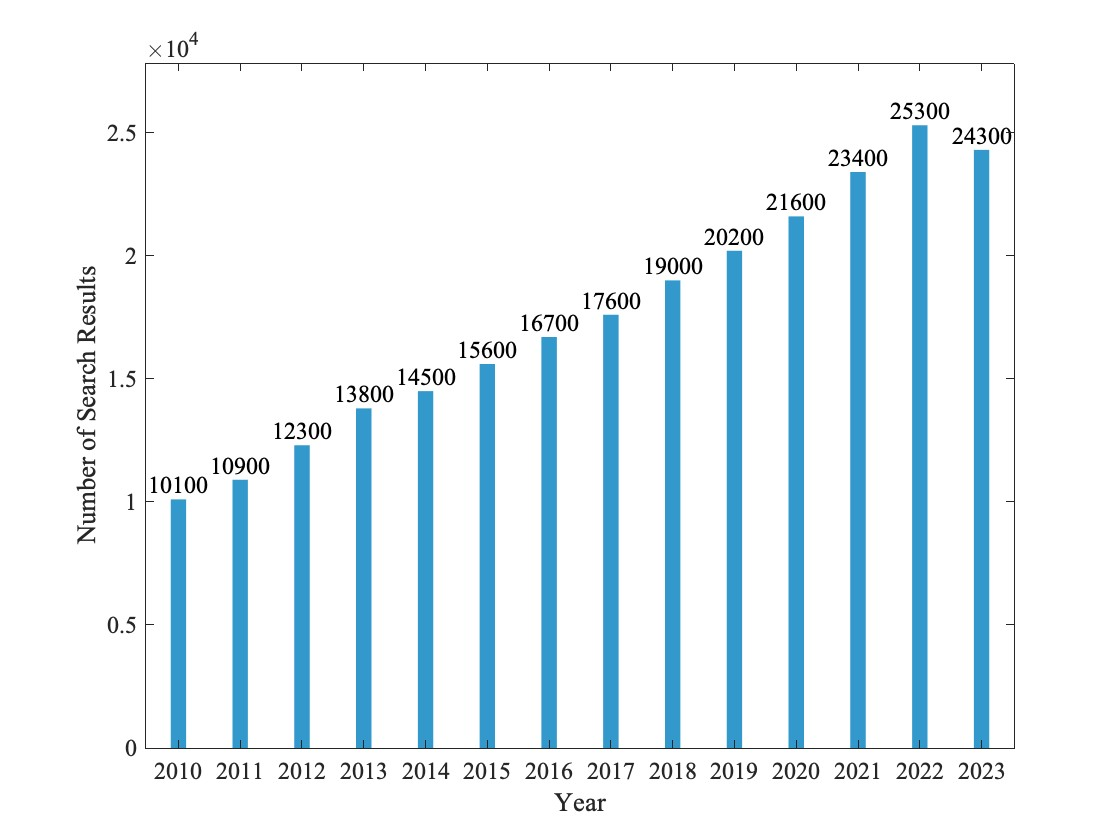
\includegraphics[width=1\textwidth]{00_Images/00_Literature_Review/00_PEMFC_July_12_2024_v1.jpg}  % Change "example-image" to the filename of your image
        \caption{This is an example image.}
        \label{fig:example1}
    \end{figure}

    \begin{figure}[H]
        \centering
        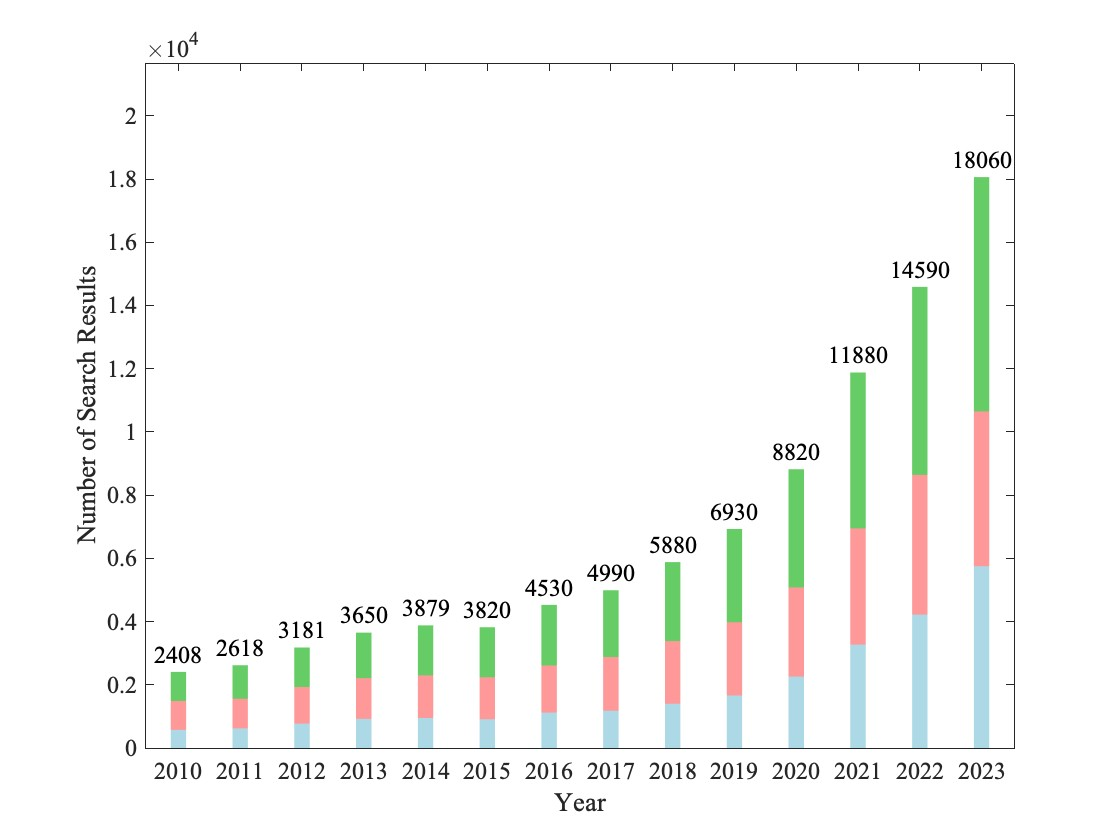
\includegraphics[width=1\textwidth]{00_Images/00_Literature_Review/00_PEMFC_ML_NN_DL_July_12_2024_v1.jpg}  % Change "example-image" to the filename of your image
        \caption{This is an example image.}
        \label{fig:example1}
    \end{figure}

\section{Relevant literature}

    Since the previous work of Yong Rui Than provides a comprehensive overview of the literature on PEMFC involving machine learning. 
    \noindent My review focused on the literature that was not covered in the previous work (i.e. 2021 - 2024). This will ensure that the literature review is up-to-date and relevant to the current state of the field.
    
    \newpage \begin{table}[H]
    \centering
    \begin{tabularx}{\textwidth}{HIJ} % Custom column widths
    \toprule
    \textbf{Title} & \textbf{Author} & \textbf{Summary} \\ 
    \midrule
    Deep learning from three-dimensional multiphysics simulation in operational optimization and control of polymer electrolyte membrane fuel cell for maximum power & Tian et al. & This study integrates an artificial neural network (ANN) with a genetic algorithm (GA) to optimize the operational control of polymer electrolyte membrane fuel cells (PEMFCs) for maximum power output. Utilizing a 3D multiphysics model, 1500 data points were generated to train the ANN, which identified a peak power density of 0.78 W/cm² at 368.8 K. The ANN-GA method effectively predicted performance and optimized conditions across temperatures from 323 K to 373 K, proving crucial for practical system design and rapid control. \\
    \midrule
    Predicting optimal membrane hydration and ohmic losses in operating fuel cells with machine learning & Paciocco et al. & This study pioneers the use of machine learning to predict optimal membrane hydration in polymer electrolyte membrane (PEM) fuel cells, focusing on high frequency resistance (HFR) and optimal hydration current density (OHCD). The long short-term memory recurrent neural network model achieved a mean absolute percentage error of 3.11\% and an R² of over 0.95 in predicting HFR, while deep learning and k-nearest neighbors models predicted OHCD with over 98\% precision and recall. These models provide robust tools for real-time parameter estimation and control, enhancing the performance and reliability of PEM fuel cells and other electrochemical devices. \\
    \midrule
    Pre-diagnosis of flooding and drying in proton exchange membrane fuel cells by bagging ensemble deep learning models using long short-term memory and convolutional neural networks & Kim et al. & This study develops a pre-diagnosis system for detecting flooding and drying in polymer electrolyte membrane fuel cells (PEMFCs) using deep learning models. The system employs long short-term memory (LSTM) and convolutional neural networks (CNN) reinforced by a bagging ensemble method, achieving detection rates of 98.52\% for flooding and 95.36\% for drying within a 30-second prediction window. Experimental data from full-scale single-cell tests, including output voltage, relative humidity, and cell temperature, were used to train the model, highlighting its potential for enhancing PEMFC stability through early fault detection. \\
    \midrule
    Machine learning modeling for proton exchange membrane fuel cell performance & Legala et al. & This study utilizes various machine learning techniques, including Artificial Neural Networks (ANN) and Support Vector Machine Regressor (SVR), to model proton exchange membrane fuel cell (PEMFC) performance and internal states. The ANN model, incorporating the dropout technique, achieved an \(R^2 \geq 0.99\) for predicting cell voltage, membrane resistance, and hydration level across different operating conditions, outperforming SVR in multivariable regression tasks. The models were developed using data from a physics-based semi-empirical model and a 1-D reduced-dimension Computational Fluid Dynamics model, demonstrating that advanced machine learning can create accurate predictive models without extensive physical experimentation. \\
    \midrule 
    \multicolumn{3}{c}{The table continues on the next page...} \\
    \bottomrule
    \end{tabularx}
    \end{table}

    \newpage \begin{table}[H]
    \centering
    \begin{tabularx}{\textwidth}{HIJ} % Custom column widths
    \toprule
    \textbf{Title} & \textbf{Author} & \textbf{Summary} \\ 
    \midrule
    Analysis and modeling of high-performance polymer electrolyte membrane electrolyzers by machine learning & Gunay et al. & This study employs box and whisker plots, principal component analysis (PCA), and classification and regression tree modeling to analyze and model high-performance polymer electrolyte membrane (PEM) electrolyzers using a database of 789 data points from 30 recent publications. The PCA identified performance risks associated with specific materials, such as cathode surfaces with high Ni content and anode surfaces with cobalt-iron alloys or RuO2. Classification trees highlighted current density, potential, and mole fractions of Ni and Co as key performance variables, while the regression tree technique accurately modeled polarization behavior with an RMSE of 0.18. \\
    \midrule 
    Machine learning optimization of operating parameters to achieve high power density and efficiency of polymer electrolyte membrane fuel cell & Kaiser et al. & This study employs five machine learning regression models—Artificial Neural Network (ANN), Decision Tree (DT), Random Forest (RF), Gradient Boosting (GB), and Extreme Gradient Boosting (xGB)—to optimize the operating parameters of polymer electrolyte membrane fuel cells (PEMFCs) for maximum power density and efficiency. Among these models, the GB regressor demonstrated the highest accuracy with an \(R^2 = 0.973\) and an \(MSE = 0.0088\) for testing data, excelling in replicating experimental polarization curves. The optimal operating conditions identified were anode and cathode pressures at 2 bar and cathode stoichiometry between 2.50–2.75, significantly enhancing PEMFC performance. The study highlights the GB model's superior capability in handling extensive datasets and optimizing complex nonlinear operational conditions, thus offering a novel approach for PEMFC performance optimization. \\
    \midrule
    A Review of physics-based and data-driven models for real-time control of polymer electrolyte membrane fuel cells & Zhao et al. & This review critically examines recent advancements in physics-based and data-driven models for the real-time control of polymer electrolyte membrane (PEM) fuel cells. Emphasizing the need for models that balance accuracy and computational efficiency, the study highlights trends such as coupling single cell models with balance-of-plant systems, incorporating aging effects for long-term predictions, and leveraging artificial intelligence algorithms for enhanced computational speed. Among the models reviewed, the study notes the superior accuracy and speed of data-driven models, particularly when trained on extensive datasets, while also addressing challenges in their applicability across diverse operational conditions. \\
    \midrule
    Application of Machine Learning in Optimizing Proton Exchange Membrane Fuel Cells: A Review & Ding et al. & This review explores the application of machine learning (ML) in optimizing proton exchange membrane fuel cells (PEMFCs) to address their cost and performance challenges for large-scale commercialization. The study highlights ML's capability to reduce experimental and computational costs by predicting outcomes based on datasets from experiments or theoretical simulations. Notable ML applications in this field include predicting active electrocatalysts, optimizing membrane electrode assemblies (MEA), designing efficient flow channels, and developing stack operation strategies. \\
    \midrule
    \multicolumn{3}{c}{The table continues on the next page...} \\
    \bottomrule
    \end{tabularx}
    \end{table}

    \newpage \begin{table}[H]
    \centering
    \begin{tabularx}{\textwidth}{HIJ} % Custom column widths
    \toprule
    \textbf{Title} & \textbf{Author} & \textbf{Summary} \\ 
    \midrule
    Towards Reliable Prediction of Performance for Polymer Electrolyte Membrane Fuel Cells via Machine Learning-Integrated Hybrid Numerical Simulations & Kaiser et al. & This study explores hybrid numerical simulations integrating machine learning (ML) to enhance the reliability and accuracy of polymer electrolyte membrane fuel cell (PEMFC) performance predictions. By addressing the limitations of existing computational fluid dynamics (CFD) models, which suffer from simplifications and inaccurate parameter approximations, the study demonstrates how ML can provide more appropriate parameters, leading to improved electrochemistry, mass/species transfer, thermal management, and water transport modeling. The ML-assisted CFD models are shown to optimize component design and material properties, significantly enhancing PEMFC efficiency and providing a robust framework for future PEMFC development and its impact on the transportation sector. \\
    \midrule
    An Optimized Data Analysis on a Real-Time Application of PEM Fuel Cell Design by Using Machine Learning Algorithms & Saco et al. & This study applies machine learning algorithms to optimize the design of polymer electrolyte membrane fuel cells (PEMFCs) by analyzing their performance under different humidity levels. Three machine learning models—Support Vector Machine Regressor (SVMR), Linear Regression (LR), and k-Nearest Neighbors (KNN)—were evaluated for their predictive accuracy using root mean square error (RMSE) as the metric. The LR model demonstrated superior performance with an RMSE of 0.0034, compared to 0.0046 for SVMR and 0.004 for KNN, effectively enhancing PEMFC efficiency through optimal humidification conditions. \\
    \midrule
    A systematic review of machine learning methods applied to fuel cells in performance evaluation, durability prediction, and application monitoring & Ming et al. & This systematic review explores the application of machine learning (ML) methods, including traditional ML and deep learning (DL), to fuel cells for performance evaluation, durability prediction, and application monitoring. The review highlights ML's effectiveness in addressing complex phenomena such as mass/heat transfer and electrochemical reactions, crucial for improving energy efficiency and durability. Notably, ML models excel in material selection, chemical reaction modeling, polarization curves, state of health monitoring, fault diagnostics, and predicting remaining useful life. The study also compares ML and DL methods, and their integration with physics simulations, providing a comprehensive outlook on future research directions for ML applications in fuel cells. \\
    \midrule
    Application of Machine Learning in Fuel Cell Research & Su et al. & This comprehensive review examines the application of machine learning (ML) algorithms in optimizing proton exchange membrane fuel cells (PEMFCs), focusing on performance prediction, service life estimation, and fault diagnosis. The study highlights the effectiveness of ML models, such as artificial neural networks (ANN), support vector machines (SVM), and random forests (RF), in solving nonlinear problems associated with PEMFCs. Notable findings include an RMSE of 0.0034 for linear regression in performance prediction, a 99\% accuracy rate in power-current curve modeling using SVM, and high precision in fault diagnosis and service life prediction. \\
    \midrule
    \multicolumn{3}{c}{The table continues on the next page...} \\
    \bottomrule
    \end{tabularx}
    \end{table}

    \newpage \begin{table}[H]
    \centering
    \begin{tabularx}{\textwidth}{HIJ} % Custom column widths
    \toprule
    \textbf{Title} & \textbf{Author} & \textbf{Summary} \\ 
    \midrule 
    Optimization of Proton Exchange Membrane Electrolyzer Cell Design Using Machine Learning & Mohamed et al. & This study leverages machine learning (ML) models, specifically polynomial and logistic regression, to optimize the design of proton exchange membrane (PEM) electrolyzer cells. By predicting eleven parameters of cell components based on four input parameters (hydrogen production rate, cathode area, anode area, and cell design type), the models achieved an average accuracy of 83.6\% and a mean absolute error (MAE) of 6.825. Validated on a test set, the ML models demonstrated excellent agreement with experimental results, showing a negligible MAE of 0.615 in hydrogen production rate predictions. The study successfully designed optimal PEM electrolyzer cells for commercial-scale hydrogen production rates (500 to 5000 mL/min), highlighting the potential of ML to significantly reduce the cost and time required for developing efficient water electrolyzers. \\
    \bottomrule
    \end{tabularx}
    \caption{Database review of literature on PEMFC and machine learning from 2021 to 2024}
    \end{table}